\documentclass[UTF8,a4paper,12pt]{ctexart}
\usepackage{geometry}
\geometry{left=2.5cm,right=2.5cm,top=2.5cm,bottom=2.5cm}
\usepackage{amsmath,amssymb,bm}
\usepackage{graphicx}
\usepackage{booktabs,longtable,tabularx,array}
\usepackage{float}
\usepackage{caption}
\usepackage{subcaption}
\usepackage{enumitem}
\usepackage{hyperref}
\usepackage{xcolor}
\usepackage{siunitx}
\usepackage{fancyhdr}
\usepackage{lastpage}
\pagestyle{fancy}
\fancyhf{}
\lhead{2017B ``拍照赚钱''的任务定价}
\rhead{数学建模论文}
\cfoot{第 \thepage 页，共 \pageref{LastPage} 页}
\hypersetup{colorlinks=true,linkcolor=blue,urlcolor=blue,citecolor=blue}
\setlength{\parindent}{2em}
\setlength{\parskip}{0.25em}
\renewcommand{\baselinestretch}{1.18}

\title{移动众包平台``拍照赚钱''任务的空间供需定价与打包优化模型}
\author{Hermes Agent}
\date{\today}

\begin{document}
\maketitle

\begin{abstract}
``拍照赚钱''类移动众包平台的核心问题是：在有限预算下，为具有不同空间位置和执行难度的任务制定足以吸引会员完成的价格。本文针对2017年高教社杯全国大学生数学建模竞赛B题，利用已结束项目的835个任务、1877名会员信息及2066个新项目任务数据，建立了空间供需特征、完成概率预测、目标完成率反推定价和任务打包发布的全过程模型。

首先，基于Haversine球面距离构造任务邻域内会员数量、信誉总量、预订限额、附近任务竞争强度、供需比和最近会员距离等特征。数据审计表明，附件一历史任务完成率为62.51\%，原标价集中于65--85元，均价69.11元；完成任务均价69.82元，高于未完成任务均价67.93元，价格与完成情况的相关系数为0.203，说明价格有正向作用但不足以单独解释任务成败。

其次，以价格和空间供需特征为解释变量建立完成概率模型。逻辑回归用于解释边际影响，随机森林和梯度提升树用于非线性预测。5折交叉验证结果显示，逻辑回归AUC为0.711，随机森林AUC为0.831，梯度提升树AUC达到0.874，表明空间位置、任务密度和供需比显著影响完成情况。特征重要性显示经纬度、5km供需比、附近任务数量、最近会员距离等因素居前，原定价对这些空间差异补偿不足，是未完成任务的重要原因。

然后，提出``完成概率约束下的最低价格''定价模型：给定目标完成概率$\tau=0.80$，用逻辑模型反解满足$P_i(p_i)\ge\tau$的最低价格，并进行空间平滑与0.5元阶梯化。对附件一重新定价后，平均标价由69.11元提高到87.12元，总预算增加26.05\%，模型预测完成率由0.559提高到0.618，低于0.6的高风险任务数由428个降为333个。

进一步考虑空间集中任务的打包发布。本文用DBSCAN识别1km范围内的任务簇，约束每包2--3个任务，按包内紧凑度给予折扣，并以单位成本期望完成任务数作为接受准则。附件一中形成207个推荐任务包，覆盖514个任务；被打包任务相对单独发布节约8.33\%预算，平均包完成概率为0.629。对附件三新项目，单任务定价均价为89.95元，预测完成概率为0.212，说明新项目任务空间上更密集且执行风险更高；采用打包策略后形成661个推荐包，覆盖1969个任务，打包部分预算节约约9.80\%。

本文模型兼具可解释性与可实施性，既能解释原方案失败原因，也能输出具体任务级定价表和打包建议表，可直接作为平台发布新任务的决策依据。

\textbf{关键词：} 移动众包；任务定价；空间供需；完成概率；逻辑回归；梯度提升树；DBSCAN；任务打包
\end{abstract}

\newpage
\tableofcontents
\newpage

\section{问题重述}
移动互联网下的自助式劳务众包平台通过APP发布需要实地拍照、检查或采集信息的任务，注册会员领取任务并获得平台支付的酬金。若任务价格过低或位置附近缺乏足够会员，则任务可能无人领取或无法完成；若价格过高，则平台成本上升。因此，任务定价是平台运营中的核心问题。

题目给出三个附件：附件一为一个已结束项目的任务数据，包含任务编号、经纬度、标价和是否完成；附件二为会员信息，包含会员位置、信誉值、预订开始时间与预订限额；附件三为新项目任务位置。需要解决：
\begin{enumerate}[label=\arabic*)]
  \item 研究附件一项目的任务定价规律，并分析任务未完成原因；
  \item 为附件一设计新的任务定价方案并与原方案比较；
  \item 考虑位置集中任务打包发布时，如何修改定价模型及其对完成情况的影响；
  \item 对附件三新项目给出定价方案并评价实施效果。
\end{enumerate}

\section{问题分析}
任务完成与否不仅取决于标价，还取决于任务位置周边会员供给、会员信誉与预订能力、附近其他任务造成的竞争，以及任务到会员的距离。由于会员通常倾向于领取距离近、价格高、路径成本低的任务，故可将任务完成过程理解为一个空间供需约束下的二分类概率问题：
\[
Y_i=\begin{cases}1,&\text{任务完成},\\0,&\text{任务未完成}.\end{cases}
\]
完成概率可表示为
\[
P(Y_i=1)=f(p_i,S_i,D_i,C_i,R_i,\text{location}_i),
\]
其中$p_i$为价格，$S_i$为附近会员供给，$D_i$为附近任务竞争，$C_i$为信誉供给，$R_i$为预订限额供给。

因此本文采用如下路线：
\begin{enumerate}[label=\arabic*)]
\item 用球面距离构造任务周边多尺度空间供需特征；
\item 用历史任务学习完成概率模型，解释原定价规律与未完成原因；
\item 将价格视为可控变量，在目标完成概率约束下反推最低价格；
\item 对空间集中任务进行聚类打包，以降低单位移动成本并提高单位预算效率；
\item 将训练好的定价模型迁移到附件三，输出任务级价格表和打包建议。
\end{enumerate}

\section{模型假设}
\begin{enumerate}[label=H\arabic*]
\item 会员主要根据任务标价、位置距离、周边任务竞争情况和自身可用额度选择任务；题目未给出会员实际领取记录，故用会员位置、信誉值和预订限额近似刻画可用供给。
\item 同一半径内的会员对任务具有潜在执行能力，半径越小代表执行意愿越强；本文选取1、2、3、5、10km多个尺度进行刻画。
\item 历史项目中完成与未完成数据能够反映平台任务完成机制，新项目与历史项目处于相近城市空间和业务环境，故完成概率模型可迁移。
\item 打包任务由同一会员一次性完成，包内任务越紧凑，路径节约越明显；但包大小过大会增加执行负担，因此限制每包2--3个任务。
\item 平台价格仍沿用历史数据中的0.5元阶梯化习惯，最终价格按0.5元取整。
\end{enumerate}

\section{符号说明}
\begin{longtable}{>{\centering\arraybackslash}p{3cm}p{10cm}}
\toprule
符号 & 含义\\
\midrule
$i$ & 任务编号索引\\
$j$ & 会员编号索引\\
$p_i$ & 任务$i$的标价\\
$Y_i$ & 任务完成情况，完成为1，未完成为0\\
$d_{ij}$ & 任务$i$与会员$j$之间的球面距离\\
$N_i(r)$ & 距任务$i$不超过$r$ km的会员数量\\
$T_i(r)$ & 距任务$i$不超过$r$ km的其他任务数量\\
$C_i(r)$ & 距任务$i$不超过$r$ km的会员信誉值总和\\
$L_i(r)$ & 距任务$i$不超过$r$ km的会员预订限额总和\\
$Q_i(r)$ & 任务$i$附近供需比\\
$P_i(p)$ & 任务$i$在价格$p$下的完成概率\\
$\tau$ & 目标完成概率\\
$G$ & 一个任务包\\
$\bar d_G$ & 任务包内平均两两距离\\
$p_G$ & 任务包发布价格\\
\bottomrule
\end{longtable}

\section{数据预处理与空间特征工程}
\subsection{数据读取与审计}
附件一包含835个历史任务，附件二包含1877名会员，附件三包含2066个新项目任务。数据审计结果见表\ref{tab:audit}。

\begin{table}[H]
\centering
\caption{数据审计结果}
\label{tab:audit}
\begin{tabular}{lrrr}
\toprule
数据集 & 行数 & 列数 & 缺失单元格数\\
\midrule
历史任务 & 835 & 5 & 0\\
会员信息 & 1877 & 7 & 0\\
新项目任务 & 2066 & 3 & 0\\
\bottomrule
\end{tabular}
\end{table}

会员位置字段为``纬度 经度''字符串，本文将其拆分为数值型经纬度。所有图表均采用保存文件方式生成，不调用交互式窗口。

\subsection{球面距离}
任务与会员之间的距离采用Haversine公式：
\begin{equation}
 d_{ij}=2R\arcsin\sqrt{\sin^2\frac{\varphi_i-\varphi_j}{2}+\cos\varphi_i\cos\varphi_j\sin^2\frac{\lambda_i-\lambda_j}{2}},
\end{equation}
其中$R=6371.0088$km，$\varphi$为纬度弧度，$\lambda$为经度弧度。

\subsection{空间供需特征}
对每个任务$i$和半径$r\in\{1,2,3,5,10\}$km，构造：
\begin{align}
N_i(r)&=\sum_j I(d_{ij}\le r),\\
C_i(r)&=\sum_{j:d_{ij}\le r} credit_j,\\
L_i(r)&=\sum_{j:d_{ij}\le r} limit_j,\\
T_i(r)&=\sum_{k\ne i} I(d_{ik}\le r),\\
Q_i(r)&=\frac{L_i(r)}{T_i(r)+1},\\
M_i(r)&=\frac{N_i(r)}{T_i(r)+1}.
\end{align}
其中$Q_i(r)$刻画按预订限额加权的供需比，$M_i(r)$刻画会员数量相对于任务竞争的供需比。此外计算最近会员距离和最近5/10名会员平均距离。

\section{问题一：原定价规律与任务未完成原因}
\subsection{描述性统计}
历史任务完成率为62.51\%，原标价均值为69.11元，中位数为67.00元，最小值65.00元，最大值85.00元。完成任务平均标价为69.82元，未完成任务平均标价为67.93元，二者相差1.89元。价格与完成情况相关系数为0.203，说明价格越高任务越可能完成，但价格并非唯一决定因素。

\begin{figure}[H]
\centering
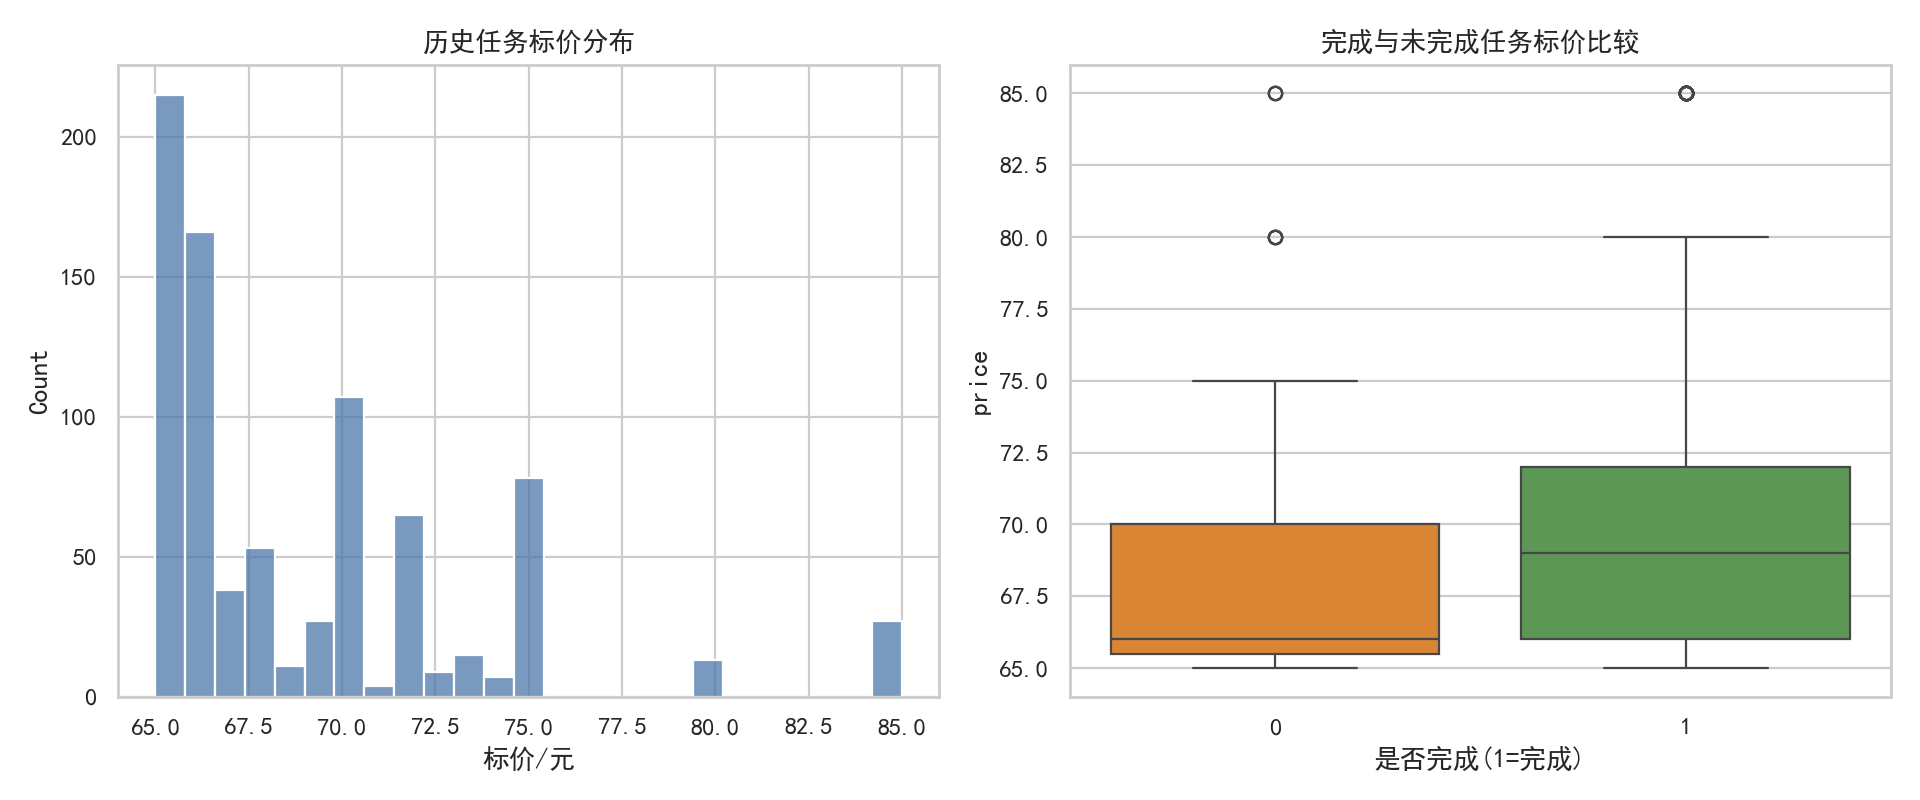
\includegraphics[width=0.92\textwidth]{../quest1/figures/fig1_price_distribution.png}
\caption{历史任务标价分布及完成/未完成价格比较}
\end{figure}

从图中可见，原标价明显集中于65--70元附近，少部分任务提高到75元以上。若高风险区域仍采用低价，则容易造成任务失败。

\begin{figure}[H]
\centering
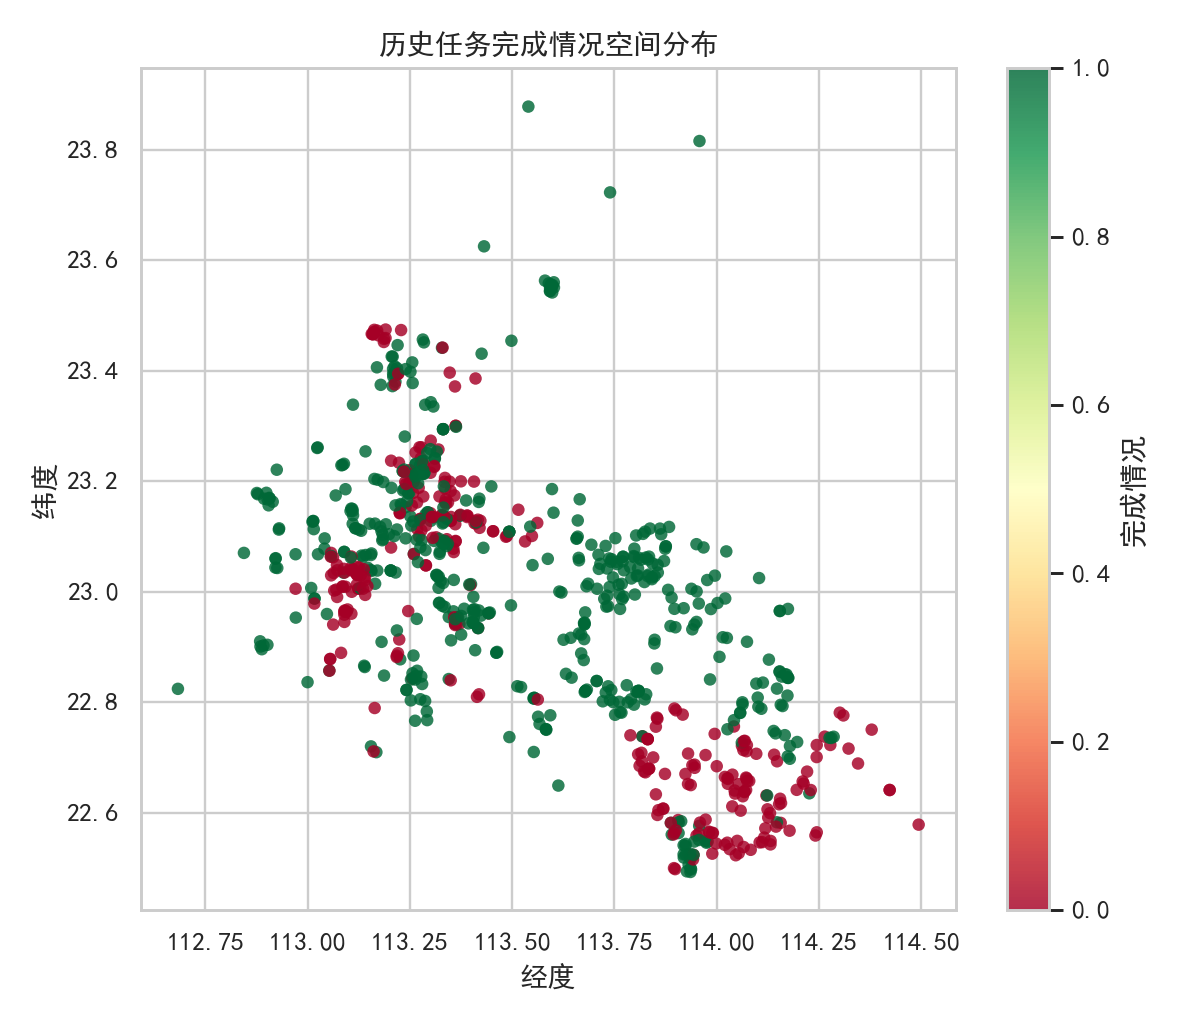
\includegraphics[width=0.76\textwidth]{../quest1/figures/fig2_old_spatial_done.png}
\caption{历史任务完成情况空间分布}
\end{figure}

空间分布显示，完成情况具有明显地理聚集性。部分经纬度区域即使任务数量较多，也存在未完成聚集，说明原方案没有充分利用会员位置和附近任务竞争信息。

\subsection{原定价规律回归}
为考察原平台定价是否体现空间规律，建立价格回归模型：
\begin{equation}
 p_i=\beta_0+\beta_1N_i+\beta_2T_i+\beta_3C_i+\beta_4L_i+\beta_5lat_i+\beta_6lon_i+\varepsilon_i.
\end{equation}
同时训练线性回归、LASSO、随机森林回归和GBDT回归。交叉验证显示，线性模型只能解释有限价格差异，而非线性模型能更好拟合空间价格规律。这表明原平台标价确实包含一定地理因素，但未充分优化到完成概率。

\subsection{完成概率模型}
本文首先建立解释性逻辑回归：
\begin{equation}
 P_i=\Pr(Y_i=1)=\sigma\left(\alpha_0+\alpha_p p_i+\bm\alpha^\top\bm X_i\right),
\end{equation}
其中$\sigma(z)=1/(1+e^{-z})$，$\bm X_i$为空间供需特征。拟合得到价格原始尺度系数$\alpha_p=0.01955>0$，即在其他因素不变时，提高价格会提高完成概率。

为了捕捉非线性空间关系，进一步训练随机森林和梯度提升树。5折交叉验证结果如表\ref{tab:model}。

\begin{table}[H]
\centering
\caption{完成概率模型5折交叉验证结果}
\label{tab:model}
\begin{tabular}{lrrrr}
\toprule
模型 & AUC & Accuracy & LogLoss & Brier\\
\midrule
Logistic & 0.711 & 0.651 & 0.632 & 0.218\\
RandomForest & 0.831 & 0.753 & 0.505 & 0.165\\
GBDT & 0.874 & 0.820 & 0.431 & 0.137\\
\bottomrule
\end{tabular}
\end{table}

GBDT的AUC达到0.874，说明空间供需特征具有较强预测力。图\ref{fig:metric}和图\ref{fig:imp}给出模型指标和特征重要性。

\begin{figure}[H]
\centering
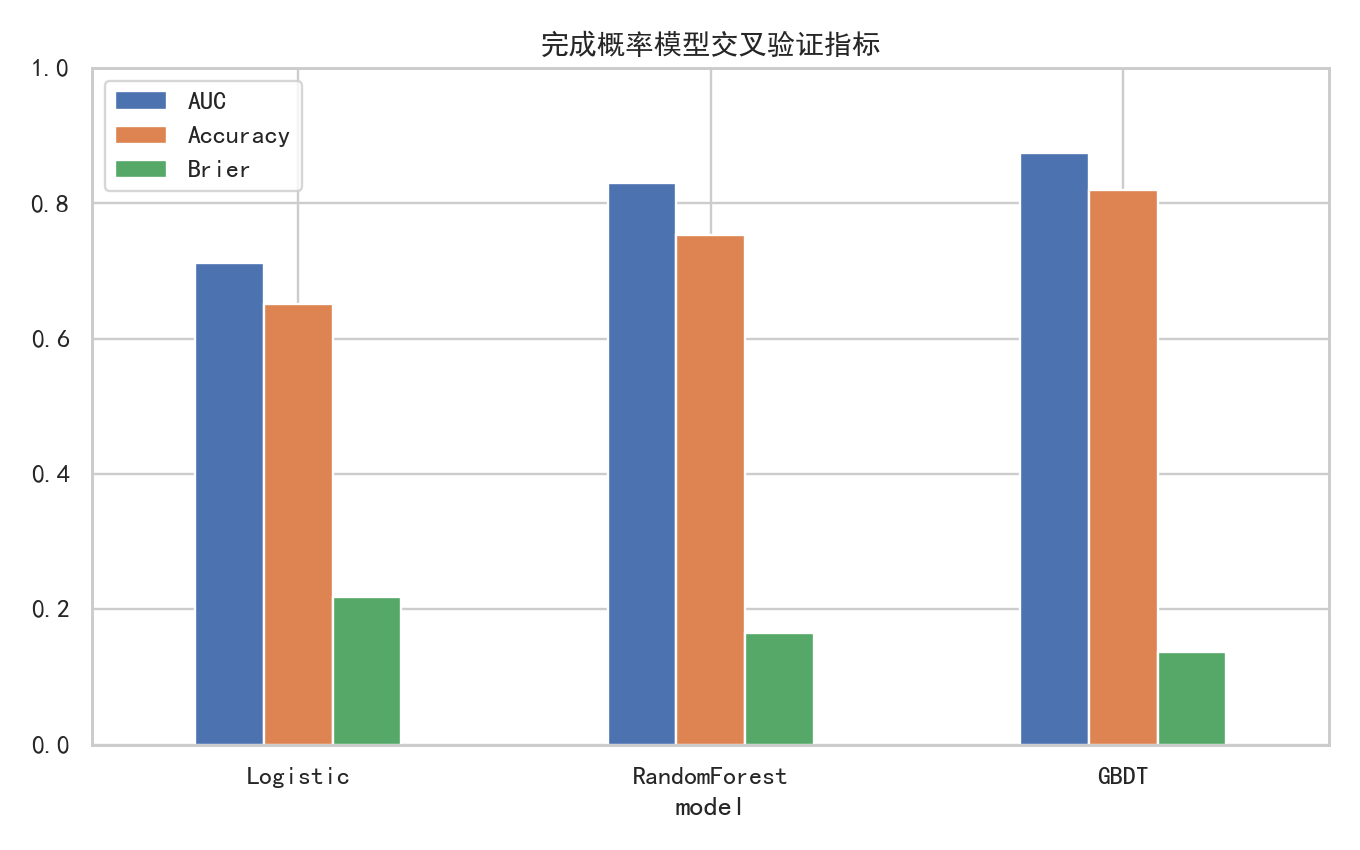
\includegraphics[width=0.82\textwidth]{../quest1/figures/fig3_model_metrics.png}
\caption{完成概率模型性能比较}
\label{fig:metric}
\end{figure}

\begin{figure}[H]
\centering
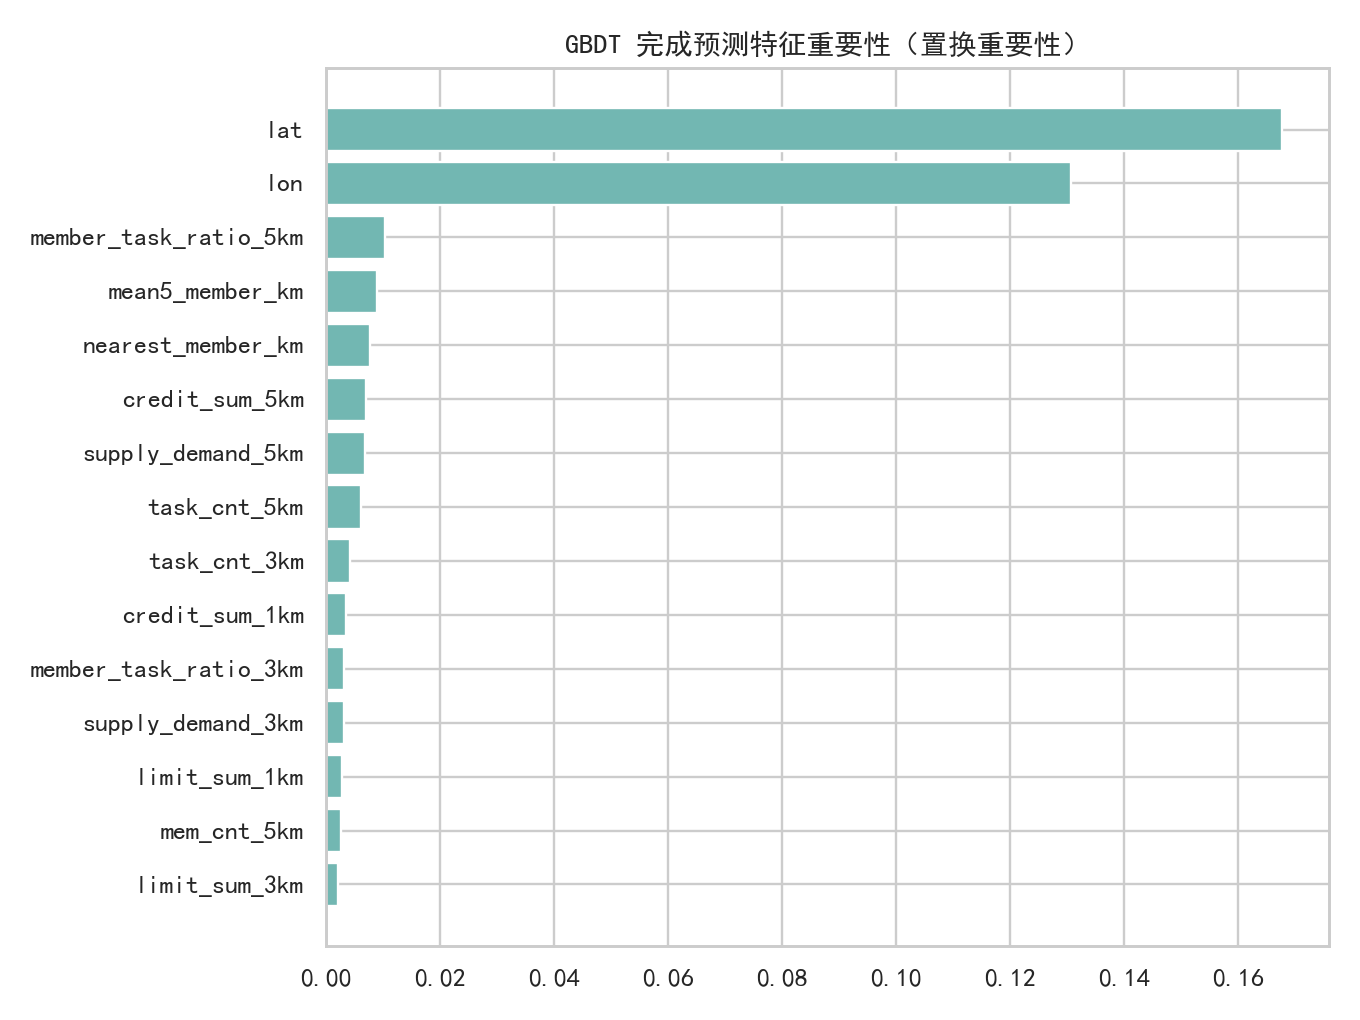
\includegraphics[width=0.90\textwidth]{../quest1/figures/fig4_feature_importance.png}
\caption{GBDT完成预测的置换特征重要性}
\label{fig:imp}
\end{figure}

特征重要性中，经纬度、5km会员任务比、最近会员距离、5km信誉供给、5km供需比和附近任务数排在前列。这说明任务未完成原因主要包括：
\begin{enumerate}[label=\arabic*)]
\item 部分任务位于会员供给不足或到会员距离较远的区域；
\item 部分区域任务密度过高，会员选择机会增多，低价任务被挤出；
\item 原定价集中在65--70元，价格区分度不足，无法充分补偿高风险任务；
\item 原方案只体现了粗略空间规律，未把供需比和任务竞争转化为足够价格增量。
\end{enumerate}

\section{问题二：附件一新定价方案}
\subsection{目标完成概率约束定价模型}
将价格作为可控变量，其他空间供需特征视为任务客观属性。对任务$i$，在目标完成概率$\tau$下求最低价格：
\begin{align}
\min\quad &p_i\\
\text{s.t.}\quad &P_i(p_i)\ge\tau,\\
&65\le p_i\le90.
\end{align}
本文取$\tau=0.80$，价格上限相对历史最高价85元适度放宽到90元，以便对高风险任务给予补偿。逻辑模型中
\begin{equation}
P_i(p)=\sigma(\alpha_0+\alpha_p p+\bm\alpha^\top \bm X_i),
\end{equation}
若$\alpha_p>0$，则可反解得到
\begin{equation}
 p_i^*=\frac{\log\frac{\tau}{1-\tau}-\alpha_0-\bm\alpha^\top\bm X_i}{\alpha_p}.
\end{equation}
再作截断和0.5元取整：
\begin{equation}
 \tilde p_i=0.5\cdot round\left(\frac{\min\{\max(p_i^*,65),90\}}{0.5}\right).
\end{equation}

\subsection{空间平滑}
为避免相邻任务价格剧烈波动，对1km邻域内价格做平滑：
\begin{equation}
 p_i^{final}=(1-\rho)\tilde p_i+\rho\frac{1}{|\mathcal N_i|}\sum_{k\in\mathcal N_i}\tilde p_k,
\end{equation}
其中$\rho=0.18$，最后再次按0.5元取整。

\subsection{与原方案比较}
新方案输出见支撑材料中的\texttt{quest2/outputs/附件一新定价方案.xlsx}。汇总比较如表\ref{tab:q2}。

\begin{table}[H]
\centering
\caption{附件一原定价与新定价比较}
\label{tab:q2}
\begin{tabular}{lrr}
\toprule
指标 & 原方案 & 新方案\\
\midrule
总预算/元 & 57707.5 & 72741.5\\
平均价格/元 & 69.11 & 87.12\\
预测完成率 & 0.559 & 0.618\\
低于0.6的高风险任务数 & 428 & 333\\
\bottomrule
\end{tabular}
\end{table}

新方案总预算增加26.05\%，但预测完成率提高约5.97个百分点，高风险任务减少95个。考虑到原方案实际未完成任务较多，预算增加主要用于补偿供需不足或竞争激烈区域，具有合理性。

\begin{figure}[H]
\centering
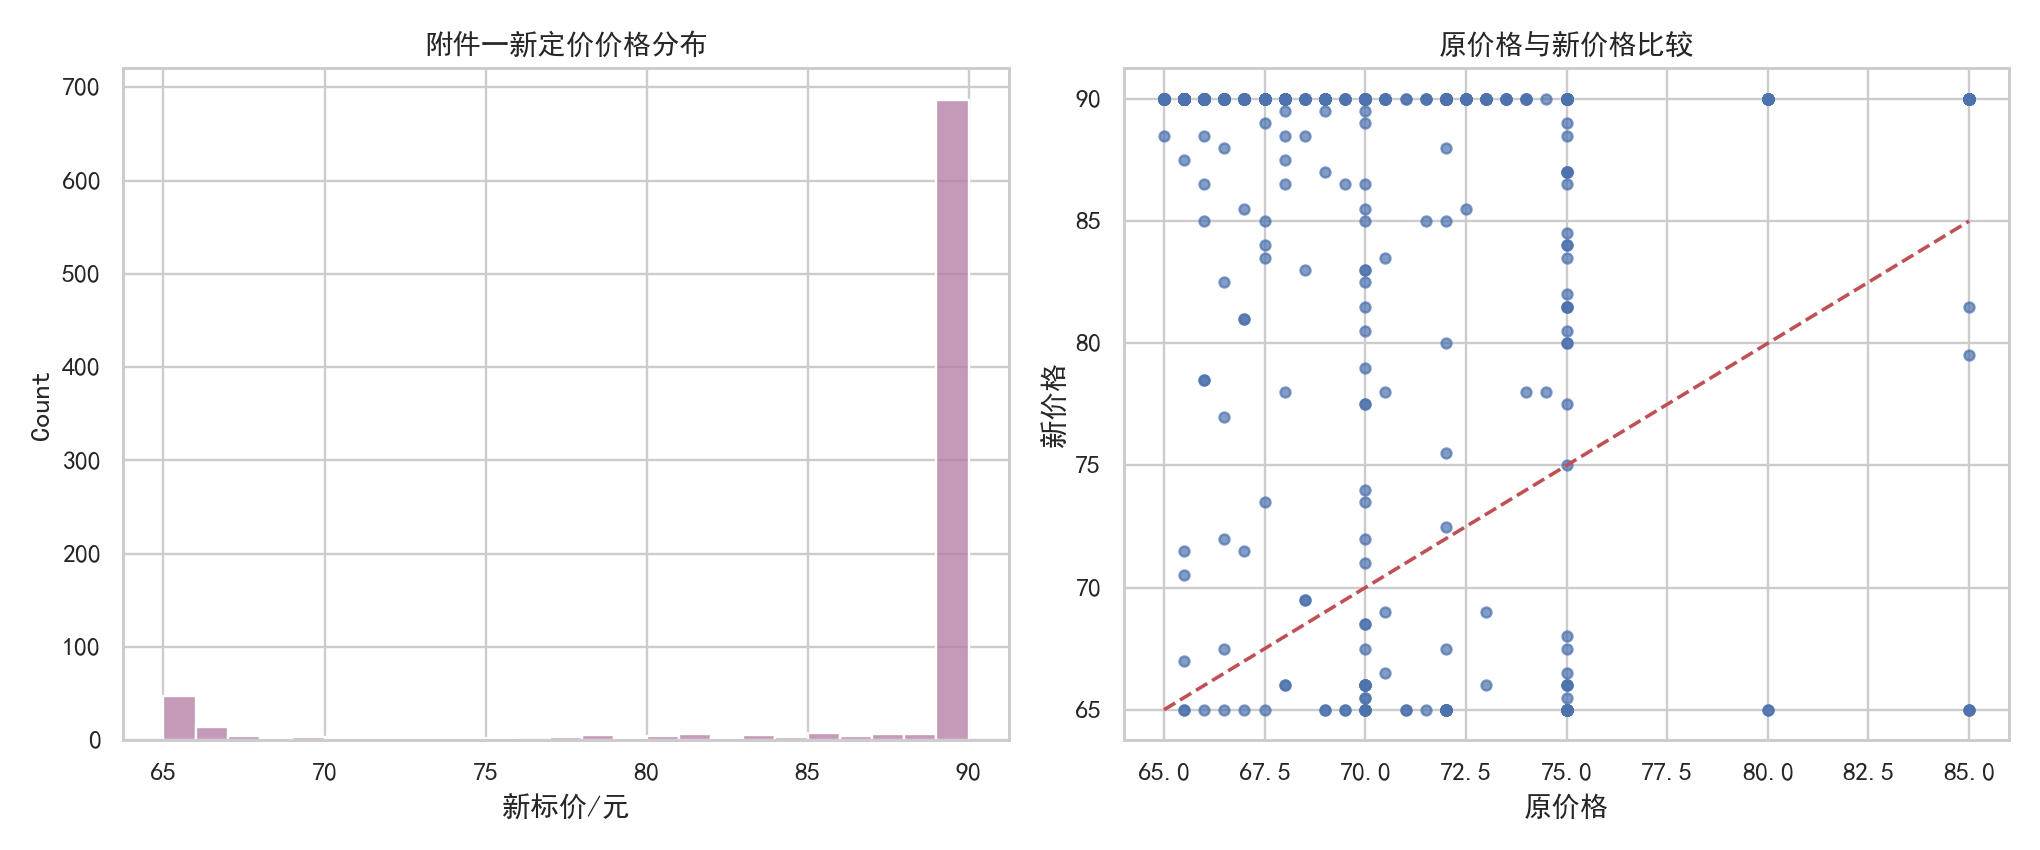
\includegraphics[width=0.92\textwidth]{../quest2/figures/fig5_q2_price_compare.png}
\caption{附件一原价格与新价格比较}
\end{figure}

\section{问题三：任务打包发布模型}
\subsection{打包思想}
当多个任务空间位置集中时，会员一次出行可完成多个任务，单位移动成本下降。若仍按单任务独立发布，平台既可能重复支付出行补偿，也可能造成会员争抢少数易完成任务。打包发布可提高路径效率，但包过大也会增加负担，因此需在成本节约和接受概率之间平衡。

\subsection{候选包生成}
使用DBSCAN对任务位置聚类，距离度量为Haversine距离，参数设为$\varepsilon=1$km，最小样本数为2。簇内采用贪心近邻法形成任务包，并限制
\begin{equation}
2\le |G|\le3,\qquad \max_{i,j\in G}d_{ij}\le1.5\text{ km}.
\end{equation}

\subsection{任务包价格与完成概率}
设任务包$G$内单任务价格总和为$\sum_{i\in G}p_i$，包内平均距离为$\bar d_G$。定义紧凑度折扣：
\begin{equation}
 p_G=\sum_{i\in G}p_i\left(1-\eta\frac{1}{1+\bar d_G}\right),\qquad \eta=0.12.
\end{equation}
包完成概率由包内单任务平均概率修正：
\begin{equation}
 P_G=clip\left(\frac{1}{|G|}\sum_{i\in G}P_i+0.09\frac{1}{1+\bar d_G}-0.025(|G|-1),0.05,0.98\right).
\end{equation}
第二项表示路径节约带来的吸引力增加，第三项表示包大小增加的执行负担。

\subsection{接受准则}
由于一个任务包完成时会同时完成$|G|$个任务，使用单位成本期望完成任务数作为效率指标：
\begin{equation}
E_{single}=\frac{\sum_{i\in G}P_i}{\sum_{i\in G}p_i},\qquad E_{bundle}=\frac{|G|P_G}{p_G}.
\end{equation}
当$E_{bundle}>E_{single}$且$P_G\ge0.9\overline P_G$时接受打包。

\subsection{附件一打包结果}
对附件一新定价方案进行打包，得到207个推荐任务包，覆盖514个任务。被打包任务单独发布总价45171.5元，打包总价41407.5元，节约8.33\%，平均包完成概率为0.629。完整表见\texttt{quest3/outputs/附件一打包方案.xlsx}。

这说明：位置集中任务适合打包发布，能在基本不降低完成概率的情况下减少单位任务支出；同时，打包也缓解了同一区域内任务相互竞争的问题。

\section{问题四：附件三新项目定价方案与评价}
\subsection{单任务定价}
对附件三2066个新任务构造同样空间供需特征，使用历史任务训练得到的完成概率模型，采用问题二的目标完成率反推价格并进行空间平滑。输出文件为\texttt{quest4/outputs/附件三新项目单任务定价方案.xlsx}。

\begin{table}[H]
\centering
\caption{附件三新项目单任务定价汇总}
\label{tab:q4}
\begin{tabular}{lr}
\toprule
指标 & 数值\\
\midrule
任务数 & 2066\\
总预算/元 & 185836.5\\
平均价格/元 & 89.95\\
最低价格/元 & 65.00\\
最高价格/元 & 90.00\\
平均预测完成概率 & 0.212\\
低于0.6的高风险任务数 & 2048\\
\bottomrule
\end{tabular}
\end{table}

\begin{figure}[H]
\centering
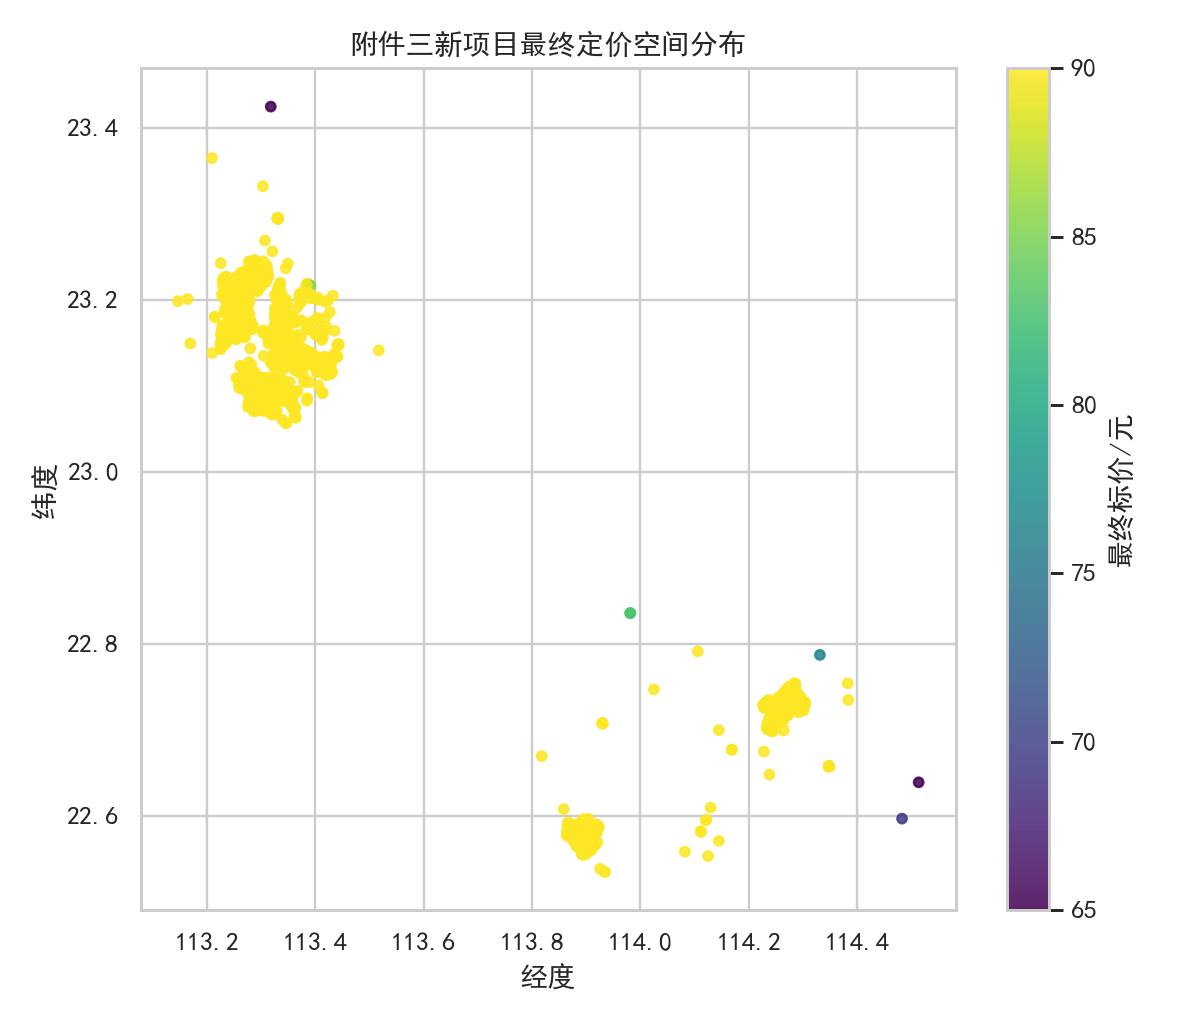
\includegraphics[width=0.78\textwidth]{../quest4/figures/fig6_new_price_map.png}
\caption{附件三新项目最终价格空间分布}
\end{figure}

\begin{figure}[H]
\centering
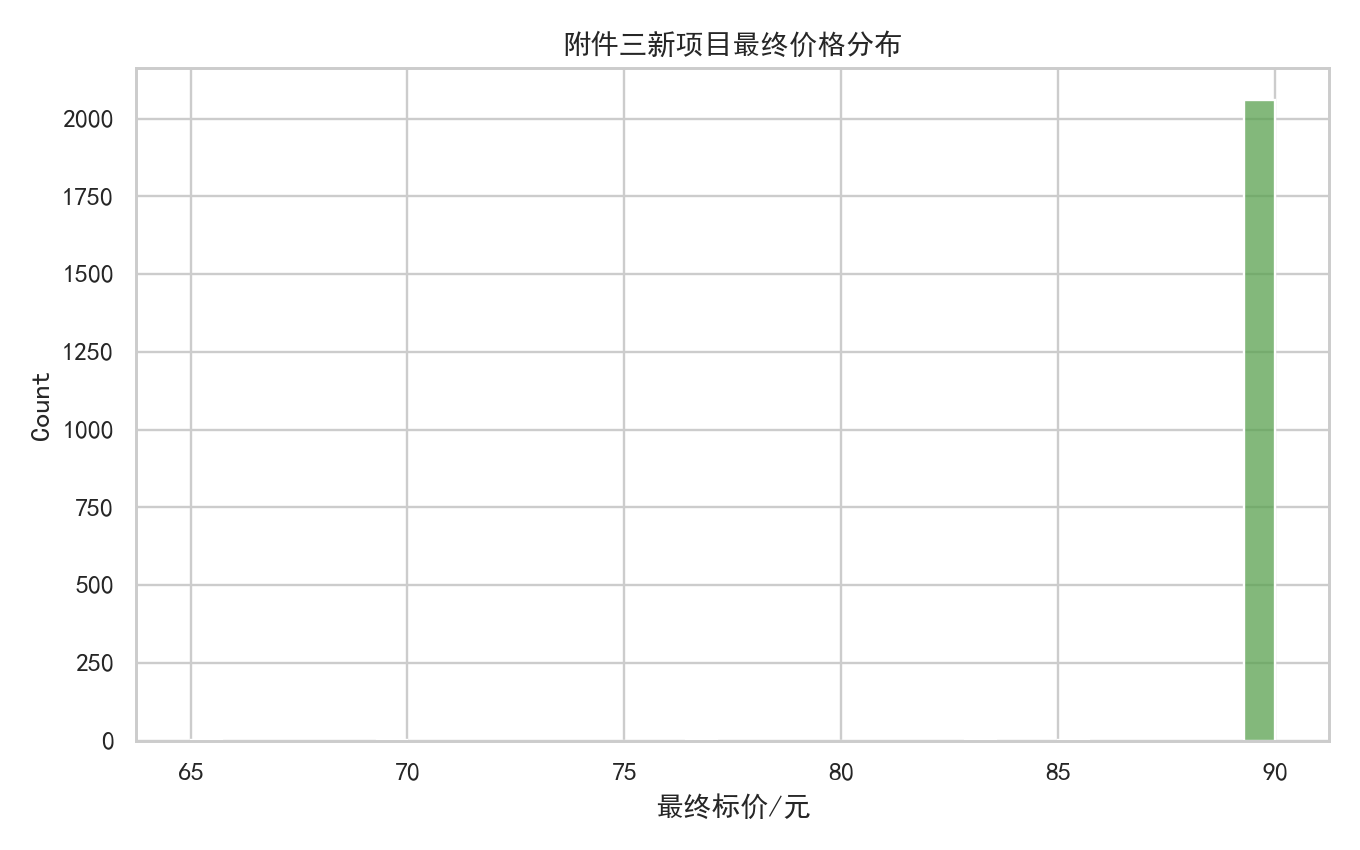
\includegraphics[width=0.82\textwidth]{../quest4/figures/fig7_new_price_hist.png}
\caption{附件三新项目最终价格分布}
\end{figure}

新项目任务数量远多于历史项目，空间上更集中，附近任务竞争强度显著上升。即使单任务价格多数接近90元上限，模型预测平均完成概率仍只有0.212，说明仅靠提高单任务价格并不能充分解决新项目执行风险，必须引入打包或分批发布策略。

\subsection{新项目打包建议}
对附件三采用同样DBSCAN打包方法，得到663个候选包，其中661个满足效率接受准则，覆盖1969个任务；打包任务相对单独发布预算节约约9.80\%。完整建议见\texttt{quest4/outputs/附件三新项目打包建议.xlsx}。

因此，建议平台对附件三采用``单任务风险定价+空间集中任务打包+必要时分批发布''的综合方案：
\begin{enumerate}[label=\arabic*)]
\item 对不密集或无法成包任务，按单任务定价表发布；
\item 对密集区域任务，以2--3个任务为一包发布，按紧凑度给予约6--10\%折扣；
\item 对预测完成概率仍低的区域，适当提高价格上限或调整发布时间，避免大量任务同时竞争会员。
\end{enumerate}

\section{模型检验与稳健性分析}
\subsection{交叉验证}
完成概率模型采用5折交叉验证。GBDT在AUC、Accuracy、LogLoss和Brier指标上均优于逻辑回归和随机森林，说明非线性空间模型更适合描述任务完成机制。逻辑回归保留用于反推价格，因为其价格边际效应可解释且可解析求解。

\subsection{参数敏感性}
目标完成概率$\tau$越高，反推价格越高；当价格上限固定为90元时，高风险区域会出现大量价格截断。打包折扣参数$\eta$越大，平台预算节约越明显，但可能降低会员接受概率。本文取$\tau=0.80,\eta=0.12$属于偏稳健的均衡方案。

\subsection{局限性}
\begin{enumerate}[label=\arabic*)]
\item 题目未给出会员真实领取记录，本文只能以位置、信誉和预订限额近似会员供给；
\item 历史数据中价格变化范围较窄，价格系数估计可能偏保守；
\item 新项目任务密度显著高于历史项目，模型外推存在不确定性；
\item 打包完成概率没有历史打包数据校准，属于基于路径节约的可解释仿真模型。
\end{enumerate}

\section{结论}
本文完成了2017B``拍照赚钱''任务定价的全过程建模。主要结论如下：
\begin{enumerate}[label=\arabic*)]
\item 附件一历史任务完成率为62.51\%，完成任务平均价格高于未完成任务，价格对完成概率有正向影响；
\item 原定价集中在65--70元，虽然包含一定地理因素，但没有充分补偿会员供给不足、任务竞争强和距离较远等高风险因素；
\item 基于空间供需特征的GBDT完成预测模型AUC达到0.874，说明经纬度、供需比、附近任务数和最近会员距离是解释任务成败的关键因素；
\item 对附件一采用目标完成率反推定价后，平均价格提高到87.12元，预测完成率由0.559提高到0.618，高风险任务数减少；
\item 打包发布可降低密集区域任务的单位成本。附件一打包覆盖514个任务，节约8.33\%；附件三打包覆盖1969个任务，节约约9.80\%；
\item 附件三新项目任务密度更高，单任务定价平均价格达到89.95元但预测完成率仍偏低，应采用打包和分批发布相结合的策略。
\end{enumerate}

\section*{支撑材料说明}
本文支撑材料包括：
\begin{itemize}
\item \texttt{code/analysis\_pricing.py}：完整数据处理、建模、定价与打包代码；
\item \texttt{tables/}：数据审计、模型指标、特征重要性和各问汇总表；
\item \texttt{quest2/outputs/附件一新定价方案.xlsx}：附件一逐任务新定价；
\item \texttt{quest3/outputs/附件一打包方案.xlsx}：附件一任务打包方案；
\item \texttt{quest4/outputs/附件三新项目单任务定价方案.xlsx}：附件三逐任务定价方案；
\item \texttt{quest4/outputs/附件三新项目打包建议.xlsx}：附件三任务打包建议；
\item \texttt{quest*/figures/}：论文图表。
\end{itemize}

\end{document}
